% !TeX root = Sprawozdanie.tex

\documentclass[12pt, a4paper]{article}
\usepackage{graphicx}
\usepackage[T1]{fontenc}
\usepackage[margin=0.75in,footskip=0.25in]{geometry}
\usepackage[polish]{babel}
\usepackage{hyperref}
\hypersetup{
    colorlinks=true,
    linkcolor=blue,
    filecolor=magenta,      
    urlcolor=blue,
    pdftitle={Overleaf Example},
    pdfpagemode=FullScreen,
    }
\graphicspath{{./plots/}}

\title{Metody numeryczne - Badanie wskaźnika giełdowego MACD}
\author{Krzysztof Nasuta, s193328}
\date{\today}

\begin{document}
\maketitle

\section{Wstęp}

\subsection{MACD}
Celem projektu jest zaimplementowanie wskaźnika giełdowego MACD (ang. Moving Average Convergence Divergence)
oraz przeprowadzenie analizy jego skuteczności. Celem wskaźnika MACD jest wykrywanie oraz rozpoznawanie
zmian trendów na rynku finansowym. MACD składa się z 2 szeregów czasowych: linii MACD oraz linii sygnałowej.
Linia MACD uzyskiwana jest jako różnica pomiędzy 2 średnimi: długoterminową oraz krótkoterminową.
Linia sygnałowa wyliczana jest jako średnia z powstałej linii MACD. Do wyliczenia średnich często
używana jest wykładnicza średnia krocząca (ang. exponential moving average, EMA). W projekcie linię MACD uzyskano jako różnicę
pomiędzy 12-dniową wykładniczą średnią kroczącą oraz 26-dniową wykładniczą średnią kroczącą. Linia sygnałowa to 
9-dniowa wykładnicza średnia krocząca z linii MACD.

Interpretacja wskaźnika MACD polega na obserwacji przecięć linii MACD oraz sygnałowej. Jeśli linia MACD przecina od dołu,
to jest to sygnał do kupna oraz zapowiedź trendu wzrostowego. Analogicznie, jeśli linia MACD przecina od góry, to jest to sygnał
do sprzedaży oraz zapowiedź trendu spadkowego. 

Aby wykluczyć fałszywe sygnały, zaimplementowano minimalną ilość dni, w których linie MACD oraz sygnałowa muszą być w trendzie,
aby sygnał został uznany za wiarygodny. Efektem ubocznym jest zmniejszenie ilości sygnałów oraz większe opóźnienie 
w reakcji na zmiany trendu.

\subsection{Implementacja}
Do Implementacji wskaźnika MACD wykorzystano język \textit{Python} oraz narzędzie 
\textit{Jupyter Notebook}, wraz z bibliotekami \textit{pandas}, \textit{numpy} oraz \textit{matplotlib}.
Dane do analizy pochodzą z serwisu \href{https://stooq.pl/}{stooq.pl}. 
W projekcie wykorzystano dane dotyczące 5 kursów walutowych:
\small
\begin{description}
    \setlength\itemsep{0.01em}
    \item[EUR/USD] \textbf{(Euro do Dolara Amerykańskiego)}
    \item[EUR/PLN] (Euro do Polskiego Złotego)
    \item[KRW/PLN] (Won Południowokoreański do Polskiego Złotego)
    \item[KRW/USD] (Won Południowokoreański do Dolara Amerykańskiego)
    \item[USD/PLN] (Dolar Amerykański do Polskiego Złotego)
\end{description}
\small
W projekcie zajmuje się głównie analizą kursu walutowego EUR/USD. Pozostałe kursy
walutowe wykorzystano do porównania skuteczności wskaźnika MACD.
Pozwala to na analizę wskaźnika MACD na różnych rynkach walutowych. 


\section{Dane wejściowe}

Dane wejściowe zawierają informacje o kursach od 01.01.2019 do 31.12.2023.

\begin{figure}[ht]
    \centering
    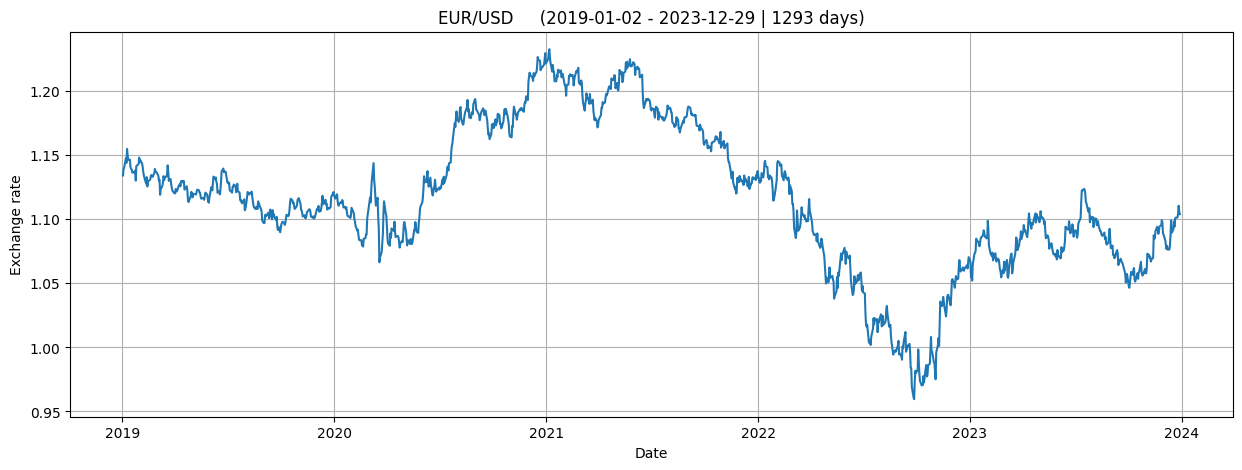
\includegraphics[width=1.0\textwidth]{eur_usd_value.png}
    \caption{Wykres kursu walutowego EUR/USD od 01.01.2019 do 31.12.2023.}
    \label{fig:eur_usd_value}
\end{figure}

\end{document}